\lhead[\chaptername~\thechapter]{\rightmark}

\rhead[\leftmark]{}

\lfoot[\thepage]{}

\cfoot{}

\rfoot[]{\thepage}

\chapter{Discussion}
\label{discussion}

\section*{Image Classification}

The evaluation of our work is done on CIFAR-10 dataset using VGG16 and MobileNet models. 
Using both models for the backbone of the hierarchical CNN, our method successfully reduced the size of the model for each user while maintaining the accuracy. 
Moreover, it can be seen that the accuracy of our method is slightly higher than the backbone networks.
The backbone networks are originally designed to classify larger classification problems with many training data. 
The reason could originate from our training method, however we used the same training scheme for all the models. 
Splitting the network into branches to obtain hierarchical network actually reduces the size of the network for each branch and make classification in each branch more suited to the task at hand, as smaller size models are more suitable with CIFAR-10 classification task.
Having said that, we believe that our hierarchical CNN could produce relatively less accuracy when it is a bigger classification task such as ImageNet. 
Accuracy is not the only concerning issue when it comes to training our model for a larger classification task. 
Another concern is that obtaining the best hierarchy would be really challenging. Further discussion about our future work will be done in the next chapter.

According to our results, both the accuracy and the memory consumption become better as the depth increases. However, further experiments should be conducted with a bigger dataset. 
Multiple smaller CNNs also showed good results as the memory consumption decreases significantly with a little drop in accuracy. 
However, the little drop in the accuracy could be significantly larger when the experiments are done on a larger dataset.

All our experiments are conducted with artificial user preferences. Even though we followed a realistic scheme, further experiments with real users are required. 

\section*{Image Retrieval}

Experiments are done with both artificial data and real-life data. 
The results with the artificial data clearly showed that our method can successfully increase the search speed by making use of user requirements.
However, the results of the experiments with the real-life data was not as good as we expected. 

There are several reasons to explain the bad performance with the real-life data. 
Sampling images from the videos is done automatically by extracting an image in every 10 seconds. 
These sampled images are both used in training phase to obtain user requirements as classification labels and in testing phase as query vectors.
However, quality of some images are bad. They are either too dark or blurred to understand. Some bad image examples can be seen in the figure \ref{fig:baddata}.

Our method depends heavily on the classification of training images to learn user requirements. 
Not only the classification accuracy is important, but also the number of classified labels has a direct effect on the search space reduction and consequently on the speed up rate.
However, pre-trained models achieve around 50\% Top-1 accuracy for the classification task on Places365 dataset.
We used pre-trained ResNet-18 architecture in our experiments and many of our training data is classified incorrectly (Figure \ref{fig:wrongly}).
Because of this, even in 426 training images, 73(out of 365) different class labels are predicted. 
While this number is too large for nearly a 1-hour video, we confirmed that there are many unrelated classification labels.

Large number of classified labels led us to limit the number of classification labels by the classification accuracy and the number of occurrences.
Unfortunately, the accuracy of our method is affected considerably.
There is a huge correlation between correctly classifying an image and correctly converting an image to its vector representation.
In our experiments, pre-trained VGG16 is used to obtain descriptor vectors from the images.
Therefore, there is a big possibility that the vectors are not representing the database images accurately.

Having said all of the above, our method is shown to perform well in ideal settings. 
Even in the worst settings, the performance of our method is similar to the baseline method. 


\begin{figure}
    \centering
    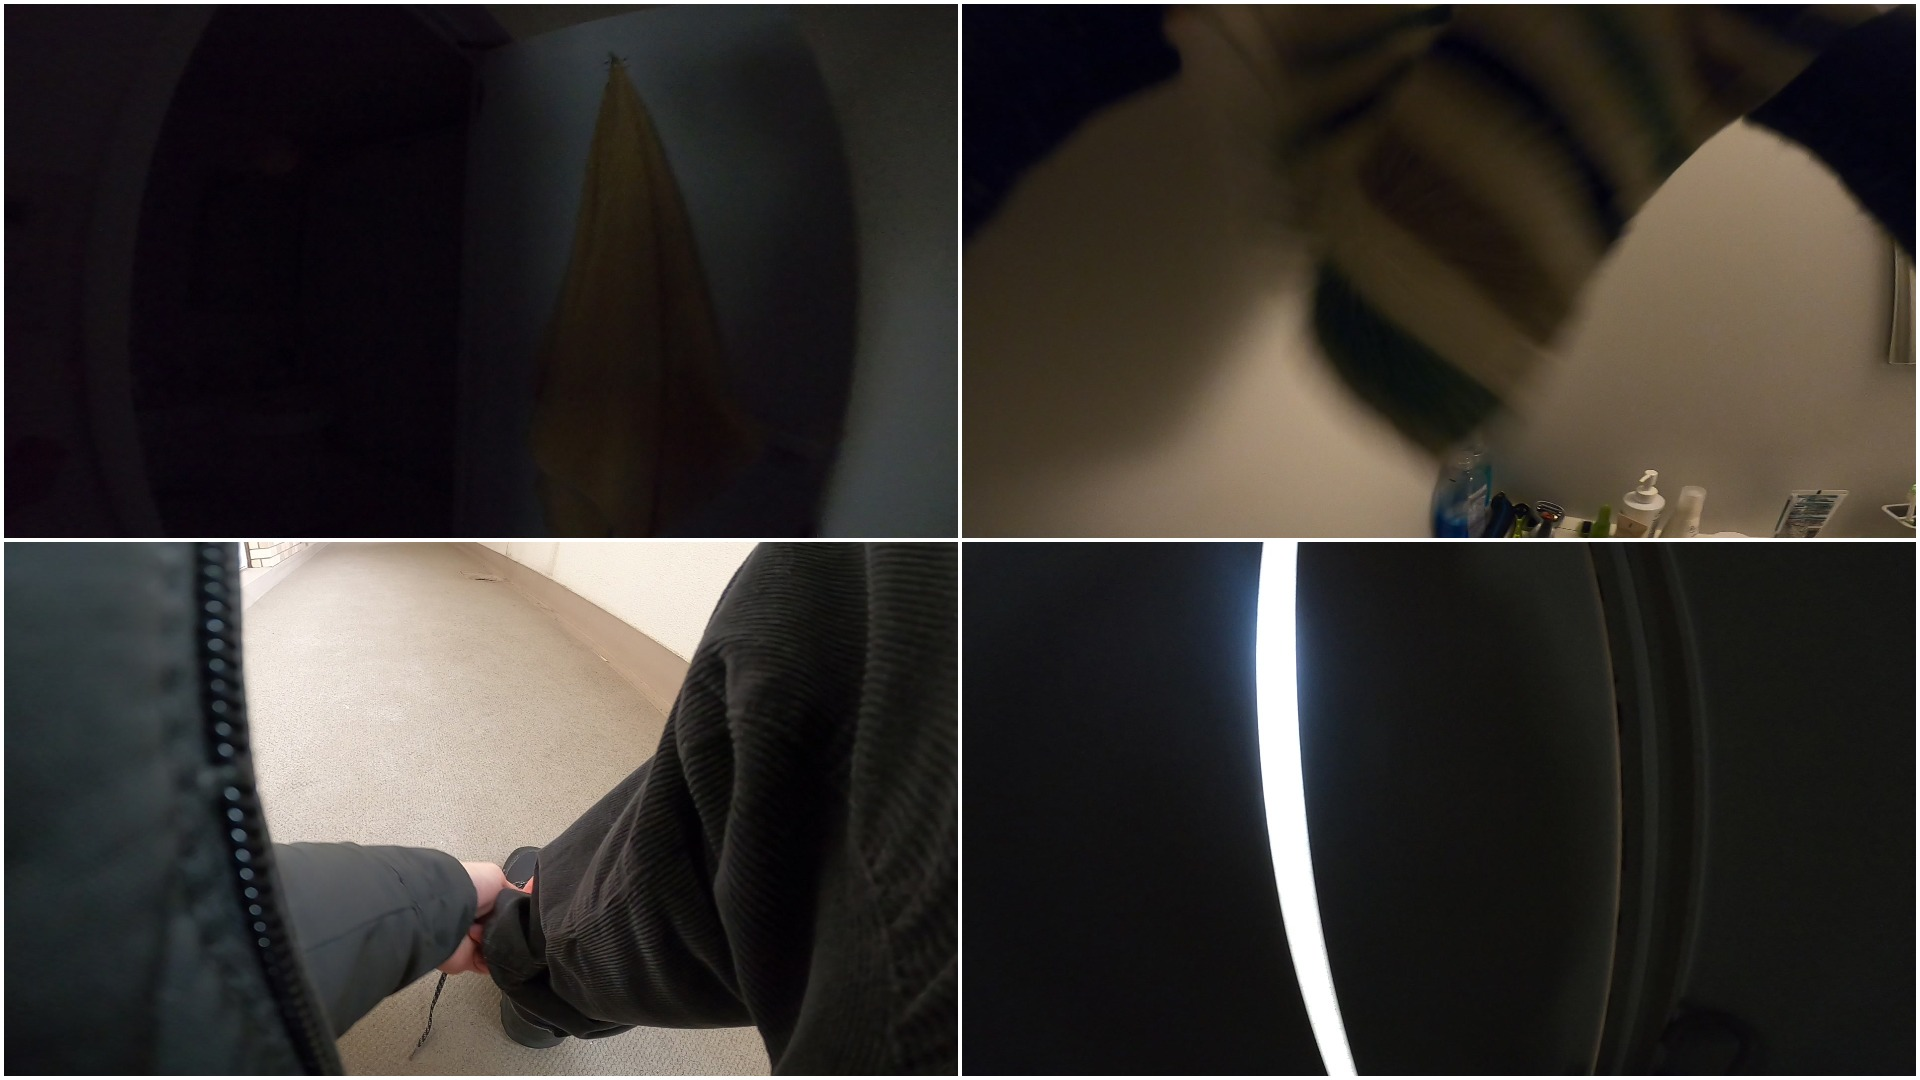
\includegraphics[width=0.8\textwidth]{thesis/images/ret-bad-images.jpg}
    \caption{Bad image examples in the test data.}
    \label{fig:baddata}
\end{figure}

\begin{figure}[ht] 
  \begin{subfigure}[b]{0.5\linewidth}
    \centering
    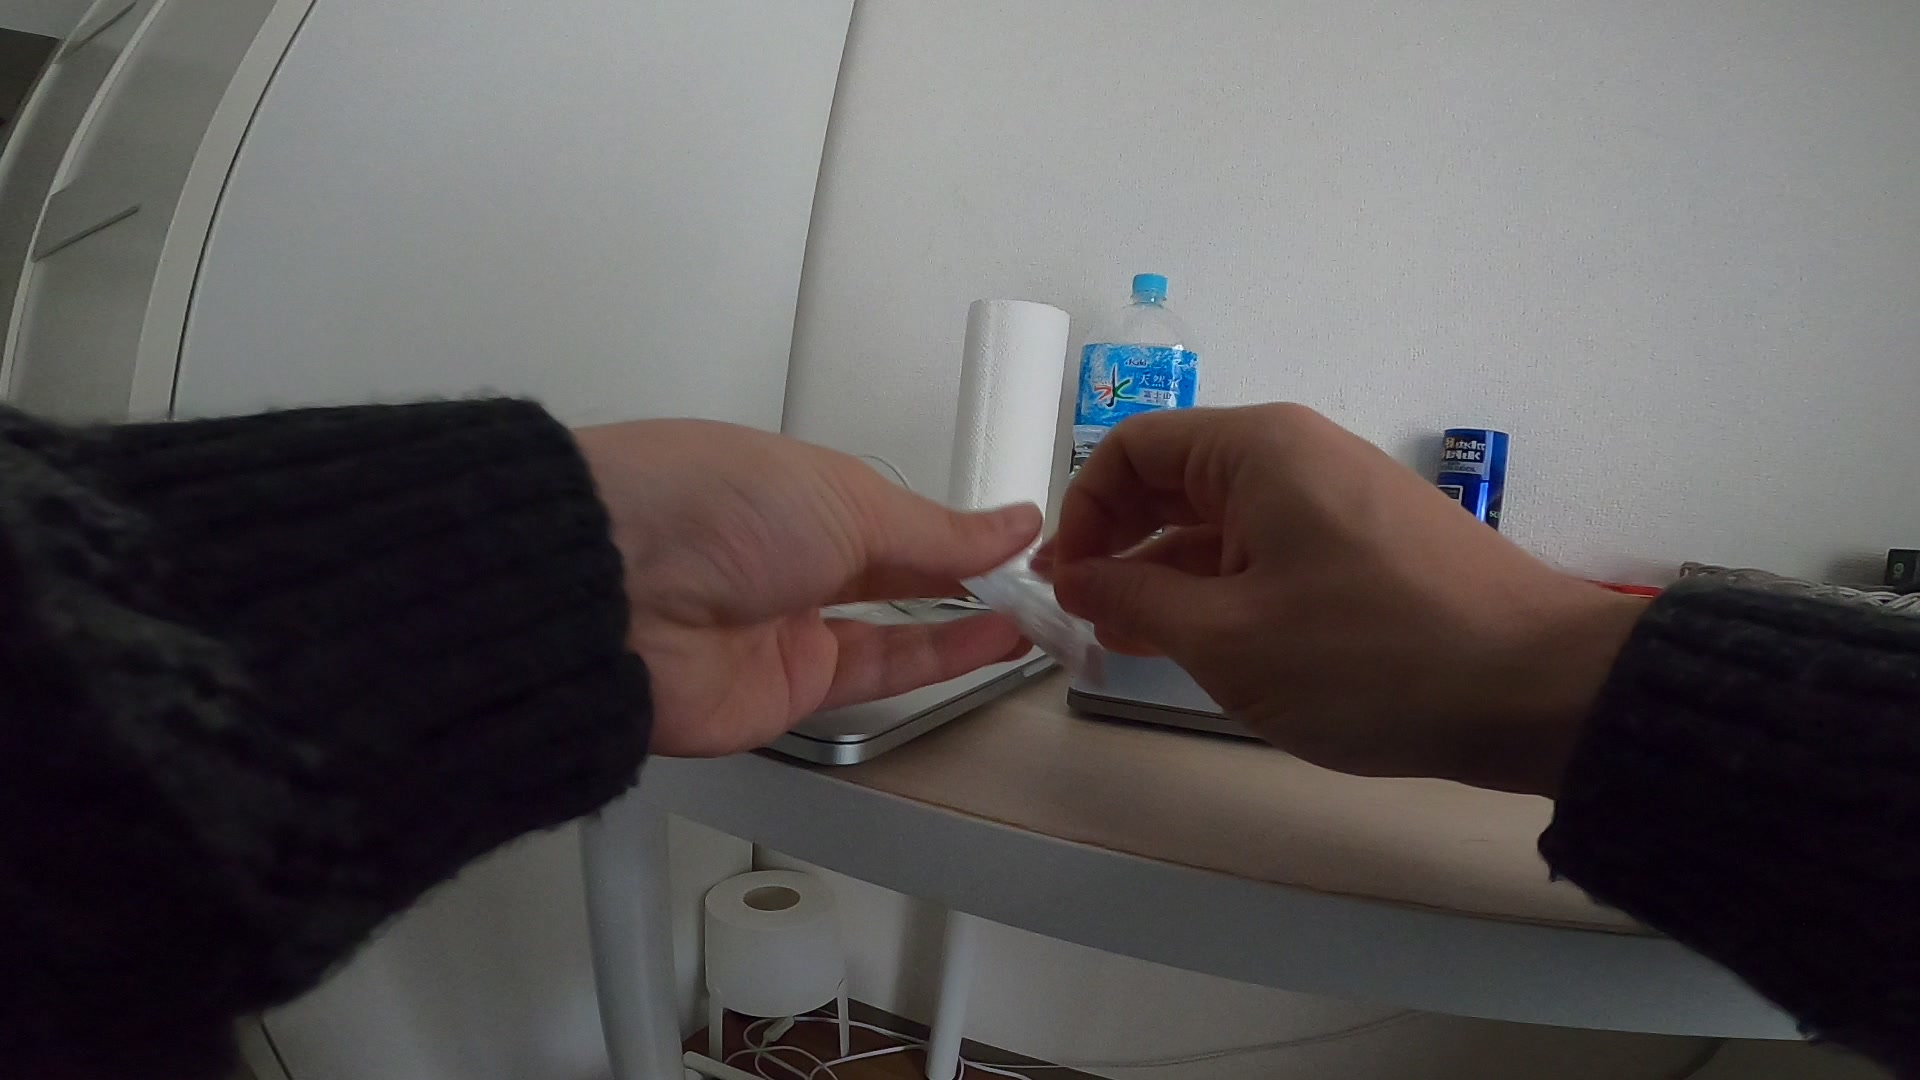
\includegraphics[width=0.75\linewidth]{{thesis/images/temp/1_beautysalon(0.63)}.jpg} 
    \caption*{Beauty Salon (63\%)}
    \vspace{4ex}
  \end{subfigure}%% 
  \begin{subfigure}[b]{0.5\linewidth}
    \centering
    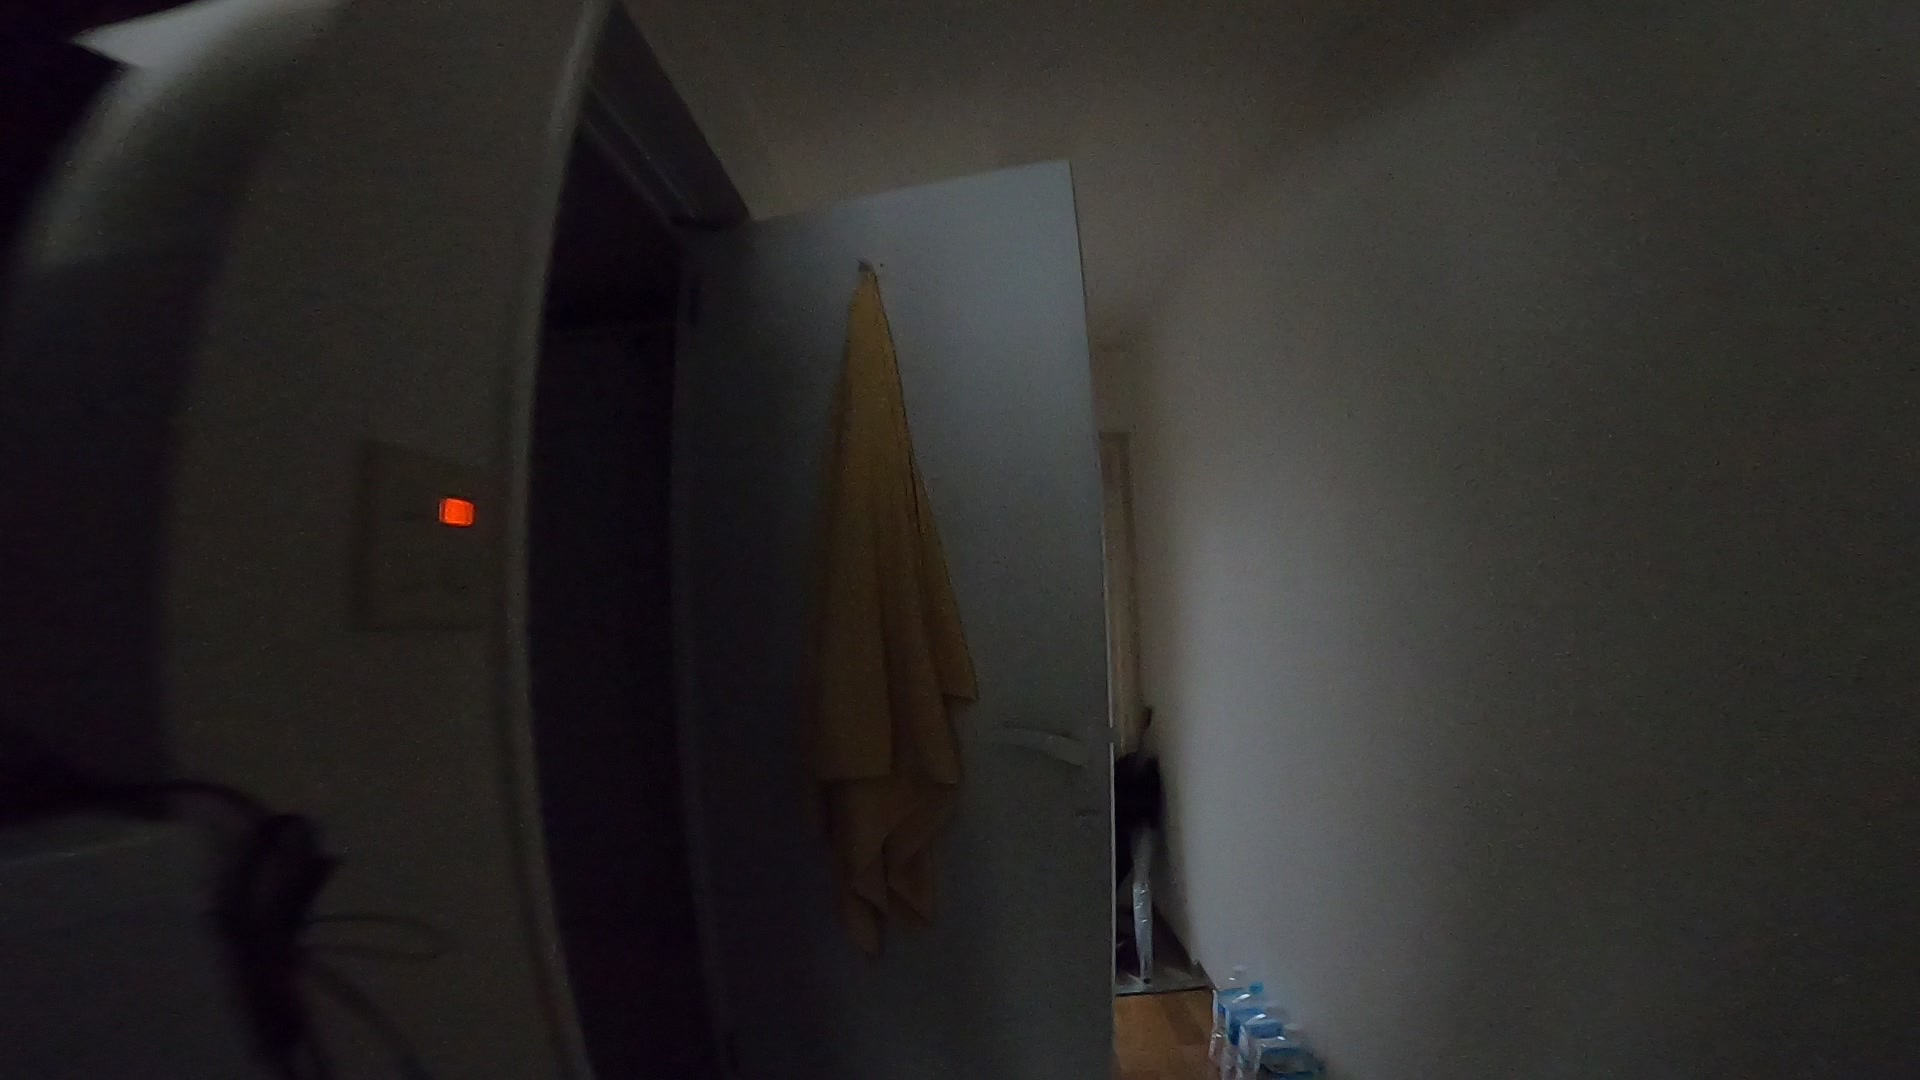
\includegraphics[width=0.75\linewidth]{{thesis/images/temp/3-alcove(0.11)}.jpg} 
    \caption*{Alcove (11\%)} 
    \vspace{4ex}
  \end{subfigure} 
  \begin{subfigure}[b]{0.5\linewidth}
    \centering
    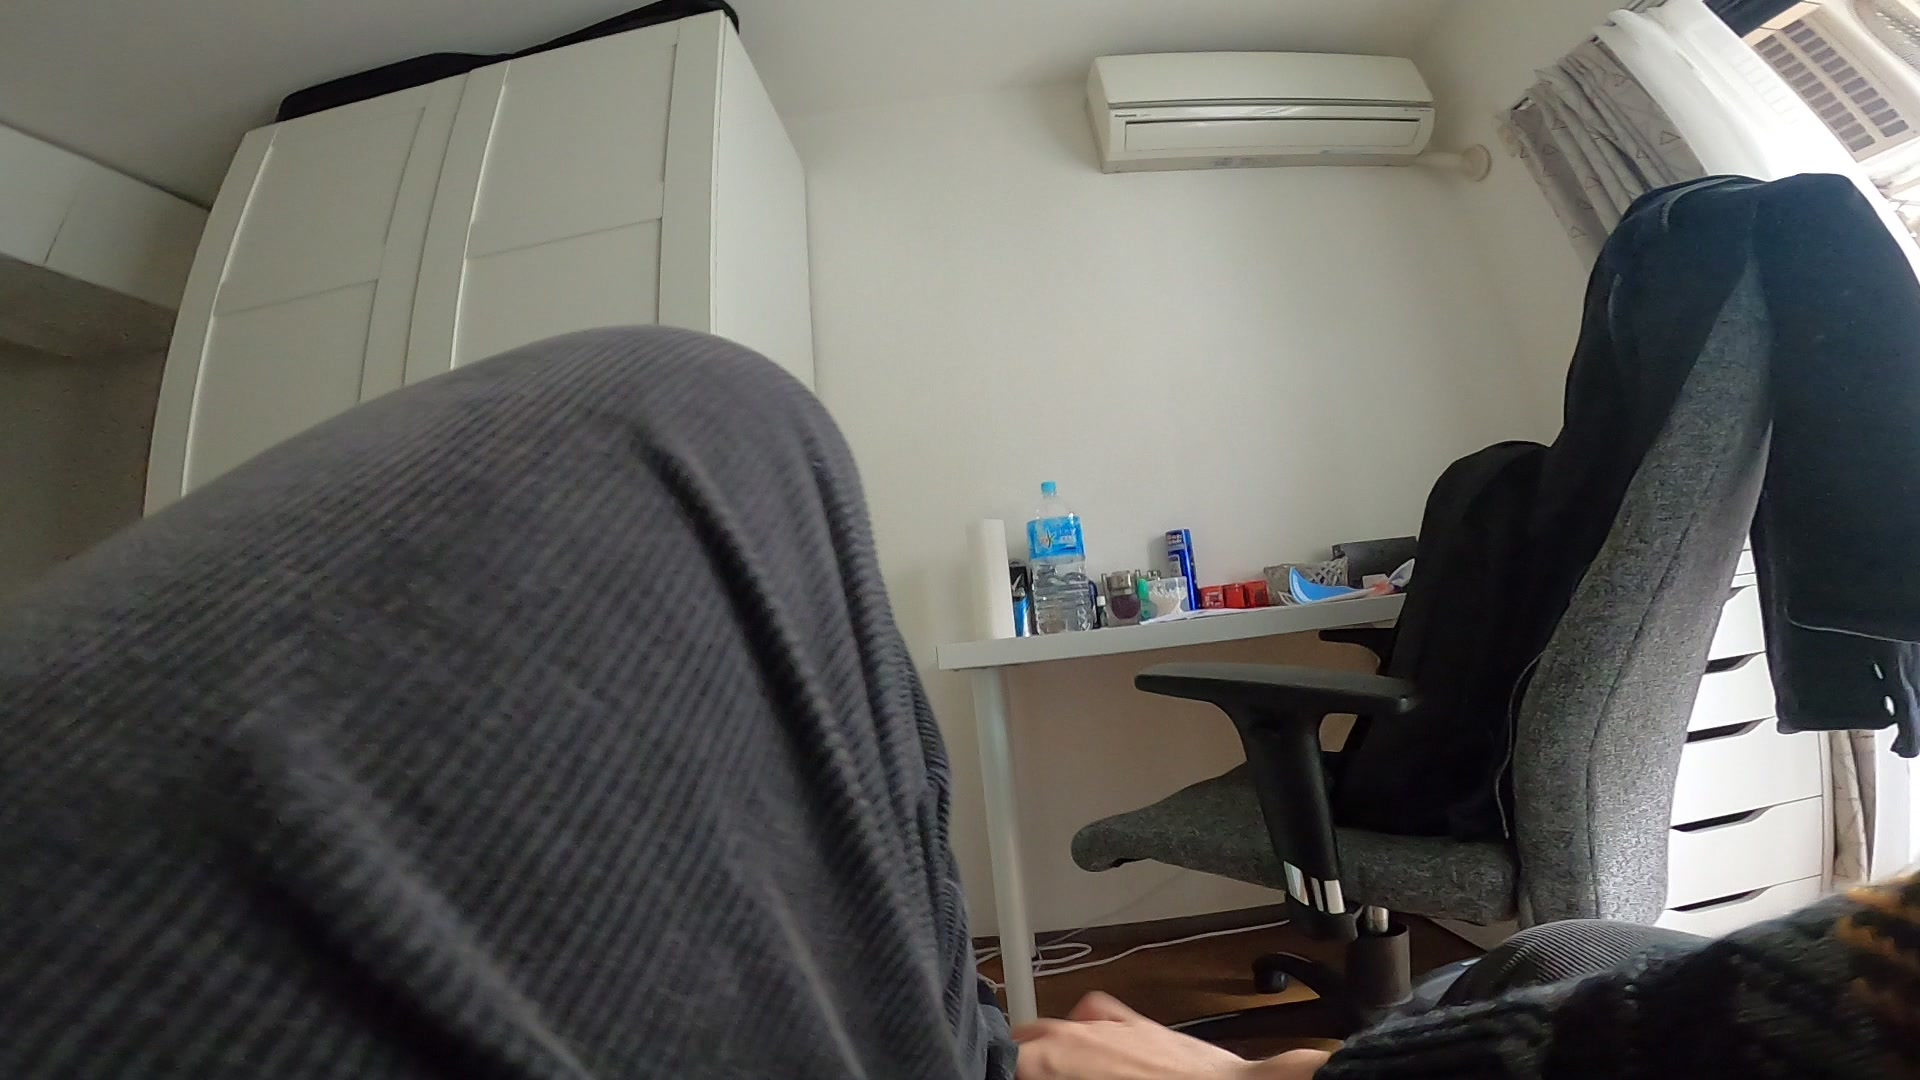
\includegraphics[width=0.75\linewidth]{{thesis/images/temp/4-airplanecabin(0.70)}.jpg} 
    \caption*{Airplane Cabin (70\%)} 
    \vspace{4ex}
  \end{subfigure}%%
  \begin{subfigure}[b]{0.5\linewidth}
    \centering
    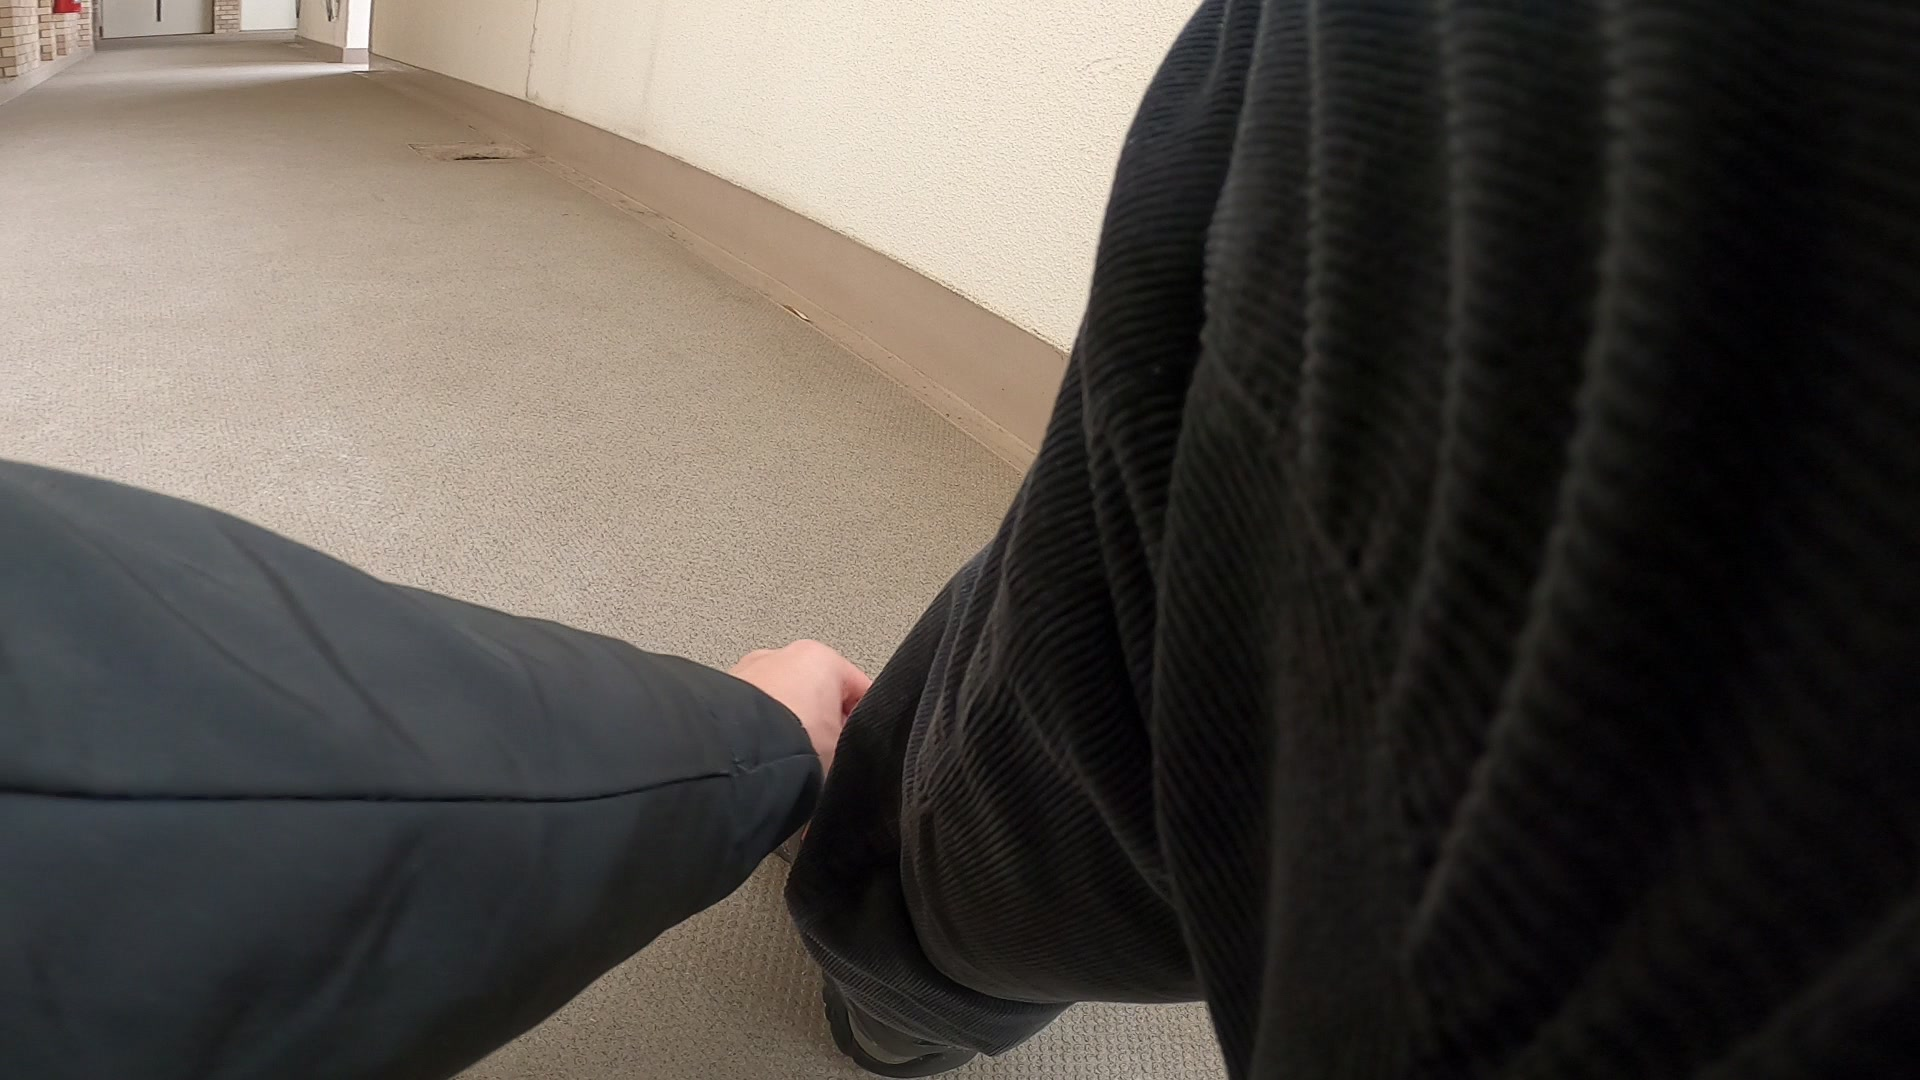
\includegraphics[width=0.75\linewidth]{{thesis/images/temp/6-berth(0.45)}.jpg} 
    \caption*{Berth (45\%)} 
    \vspace{4ex}
  \end{subfigure} 
  \begin{subfigure}[b]{0.5\linewidth}
    \centering
    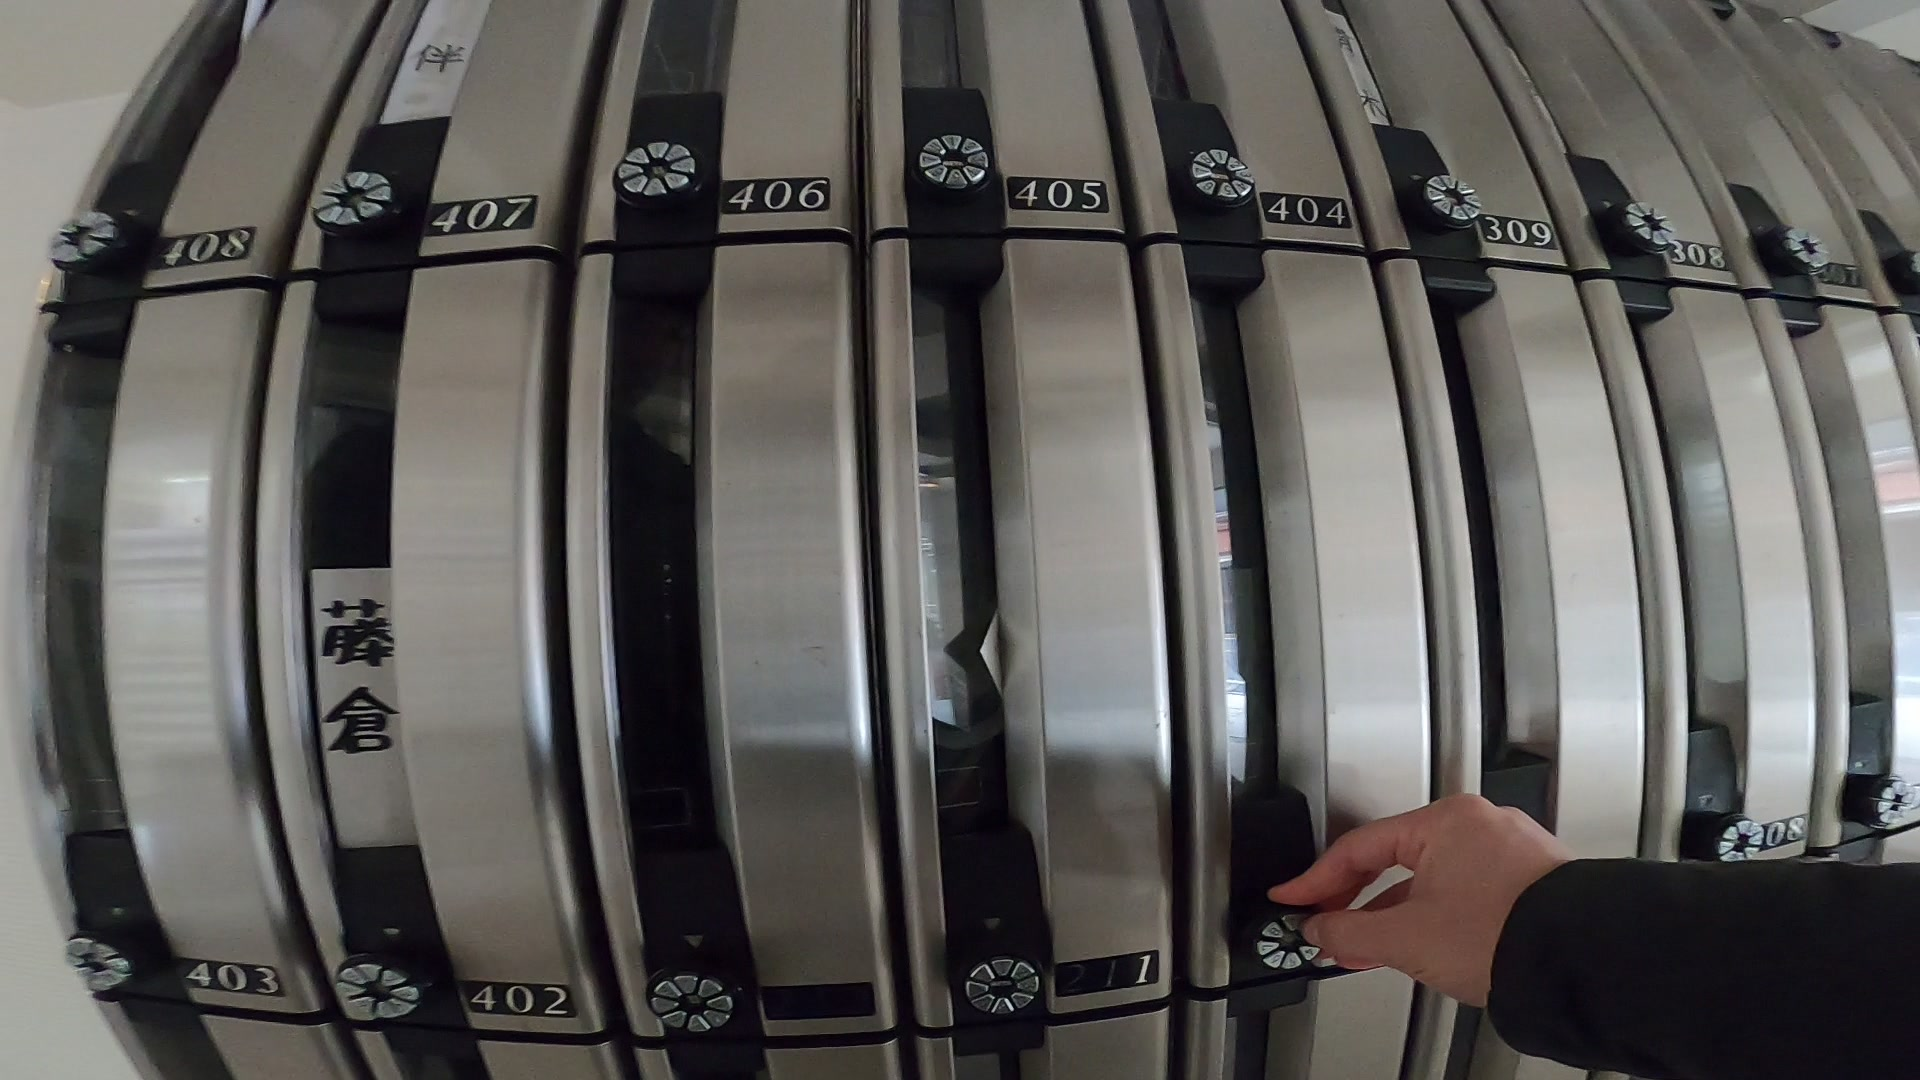
\includegraphics[width=0.75\linewidth]{{thesis/images/temp/7-serverroom(0.25)}.jpg} 
    \caption*{Server Room (25\%)} 
  \end{subfigure}%%
  \begin{subfigure}[b]{0.5\linewidth}
    \centering
    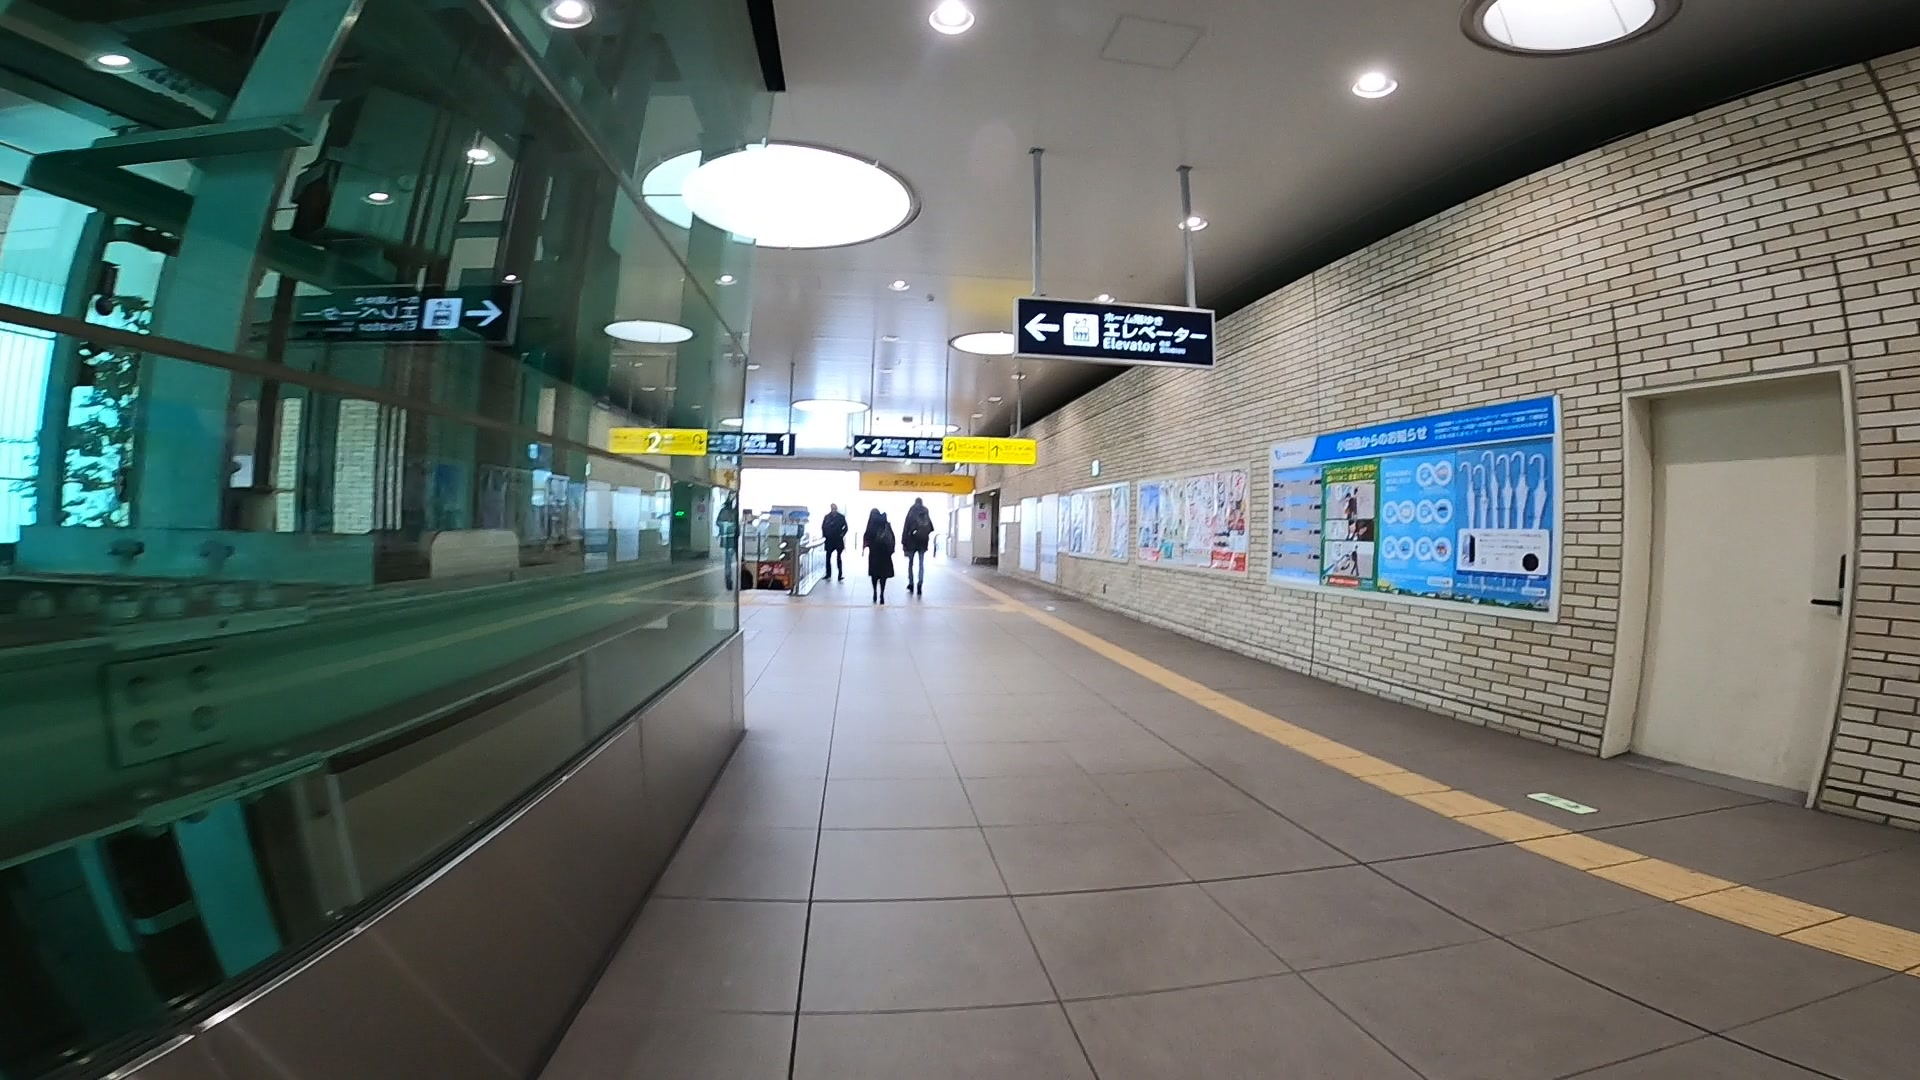
\includegraphics[width=0.75\linewidth]{{thesis/images/temp/9-airportterminal(0.82)}.jpg} 
    \caption*{Airport Terminal (82\%)}
  \end{subfigure} 
  \caption{Illustration of images with wrong classification}
  \label{fig:wrongly} 
\end{figure}
